%\documentclass[onecolumn]{IEEEtranTIE}
\documentclass[journal]{IEEEtranTIE}
\usepackage{graphicx}
\usepackage[noadjust]{cite}
\usepackage{picinpar}
\usepackage{amsmath}
\usepackage{stfloats}
%%\usepackage{dblfloatfix}
\usepackage{url}
\usepackage{flushend}
\usepackage[latin1]{inputenc}
\usepackage{colortbl}
\usepackage{soul}
\usepackage{multirow}
\usepackage{pifont}
\usepackage{color}
\usepackage{alltt}
\usepackage[hidelinks]{hyperref}
\usepackage{enumerate}
\usepackage{siunitx}
\usepackage{breakurl}
\usepackage{epstopdf}
\usepackage{pbox}

%% My packages
%% \usepackage[cmex10]{amsmath}
%% \interdisplaylinepenalty=2500
\usepackage{algpseudocode}
%% \usepackage{array}
\usepackage[caption=false,font=footnotesize]{subfig}

\usepackage{tikz}
\usetikzlibrary{arrows.meta}
%% \usepackage{mathabx}


\newcommand{\hide}[1]{\ignorespaces}
\newcommand{\jx}[1]{{\bf Jiaxiang: }#1{ \bf End}}
\newtheorem{theorem}{Theorem}
\newtheorem{lemma}[theorem]{Lemma}
\newtheorem{definition}[theorem]{Definition}

% Define the fontsize in environment {verbatim}
\makeatletter
\def\verbatim{\small\@verbatim \frenchspacing\@vobeyspaces \@xverbatim}
%\def\verbatim@font{\small\ttfamily}
\makeatother

\usepackage{microtype}


\begin{document}
\title{Formal Modeling and Verification of a Rate-Monotonic Scheduling Implementation with Real-Time Maude}

\author{
  \vskip 1em
  Jiaxiang~Liu,
  Min~Zhou,
  Xiaoyu~Song, \emph{Member}, \emph{IEEE},
  Ming~Gu,
  and Jiaguang~Sun

  \thanks{
    Manuscript received November 8, 2015; revised March 30, 2016 and
    July 13, 2016; accepted October 20, 2016. This work was supported
    in part by NSFC Program (No. 91218302, No. 61527812), National
    Science and Technology Major Project (No. 2016ZX01038101), MIIT
    IT funds (Research and application of TCN key technologies) of
    China, and The National Key Technology R\&D Program
    (No. 2015BAG14B01-02).

    J. Liu is with the Department of Computer Science \& Technology,
    Tsinghua University, Beijing 100084, China, and also with LIX,
    \'Ecole Polytechnique, Palaiseau 91120, France (e-mail:
    jiaxiang.liu@hotmail.com).

    M. Zhou is with the School of Software, Tsinghua University,
    Beijing 100084, China (corresponding author; phone:
    +86-xxx-xxxx-xxxx; fax: xxx-xxxx-xxx; e-mail: zhoumin@gmail.com).

    X. Song is with the Department of Electrical \& Computer
    Engineering, Portland State University, Portland, OR 97207-0751,
    USA.

    M. Gu and J. Sun are with the School of Software, Tsinghua
    University, Beijing 100084, China.
  }
}

\maketitle
	
\begin{abstract}
Rate-monotonic scheduling (RMS) is one of the most important real-time
scheduling used in industry. There are a large number of results about
RMS, especially on its schedulability. However, the theoretical
results do not contain enough details to be used directly for an
industrial RMS implementation. On the other hand, the correctness of
such an implementation is of the crucial importance. In this paper, we
analyze a realistic RMS implementation by using Real-Time Maude, a
formal modeling language and analysis tool based on rewriting
logic. Overhead and some details of the hardware are taken into
account in the model. We validate the schedulability and the
correctness of the implementation within key scenarios. The soundness
and the completeness of our approach are substantiated.
\end{abstract}

\begin{IEEEkeywords}
Embedded systems, formal verification, modeling, real-time systems,
rewriting logic, scheduling.
\end{IEEEkeywords}

\markboth{IEEE TRANSACTIONS ON INDUSTRIAL ELECTRONICS}%
{}

\definecolor{limegreen}{rgb}{0.2, 0.8, 0.2}
\definecolor{forestgreen}{rgb}{0.13, 0.55, 0.13}
\definecolor{greenhtml}{rgb}{0.0, 0.5, 0.0}


\section{Introduction}\label{s:introduction}

\IEEEPARstart{P}{eriodic} task scheduling is one of the most important
topics within the field of industrial real-time systems. A set of
periodic tasks is said to be \emph{schedulable} with respect to some
scheduling algorithm if all jobs meet their
deadlines. \emph{Rate-monotonic scheduling} (\emph{RMS}) is a
\emph{fixed} priority scheduling algorithm for preemptive hard
real-time environments proposed by Liu and
Layland~\cite{DBLP:journals/jacm/LiuL73}, which assigns priorities to
jobs according to the periods of
the
corresponding tasks: the smaller
period, the higher priority. RMS is proven to be the \emph{optimal}
fixed priority scheduling algorithm~\cite{DBLP:journals/jacm/LiuL73},
in the sense that any set of tasks, which is schedulable under
\emph{some} fixed priority scheduling algorithm, is also schedulable
with respect to RMS. It is widely used in safety-critical real-time
applications, such as vehicles and avionics, thanks to its optimality
and easiness to implement.

Liu and Layland~\cite{DBLP:journals/jacm/LiuL73} gave a sufficient
condition for the schedulability of a set of $n$ tasks scheduled by
RMS: $\displaystyle\Sigma^n_{i=1}C_i/T_i \le n(2^{1/n}-1)$, where
$C_i$ and $T_i$ are the \emph{computation (time) requirement} and the
period of task $\tau_i$, respectively. Two main directions on RMS have
been explored since then. One is to relax the assumptions on the
original RMS model, making it applicable on more systems.  For
instance,
\cite{DBLP:conf/rtss/LehoczkySS87,DBLP:journals/rts/SpruntSL89,DBLP:conf/rtss/LehoczkyR92,DBLP:journals/tc/StrosniderLS95}
allow aperiodic tasks in the scheduling,
\cite{DBLP:journals/pe/LeungW82,audsley1993deadline} generalize RMS to
be \emph{deadline-monotonic}, \cite{DBLP:journals/tc/ShaRL90} allows
resource sharing among tasks,
\cite{dhall1978real,DBLP:journals/rts/LopezGDG03,DBLP:journals/tpds/LopezDG04,DBLP:journals/tc/BaruahG03}
extend RMS on multiprocessors, and
\cite{DBLP:journals/rts/OhS94,DBLP:journals/rts/GhoshMMS98,DBLP:journals/tpds/BertossiMR99}
enhance fault-tolerance. The other direction is to generate better
schedulability test conditions for the algorithm and its
extensions~\cite{DBLP:conf/rtss/LehoczkySD89,DBLP:conf/rtss/KuoM91,DBLP:journals/tc/BiniBB03,DBLP:journals/rts/LopezGDG03,DBLP:journals/tc/BaruahG03,gardner1999}. The
RMS algorithm is no doubt of practical importance.

It is even more crucial to ensure the reliability of an implementation
instead of the algorithm, when RMS serves in a safety-critical
system. When analyzing a realistic implementation, theoretical results
may be no more applicable. For instance, even though the conditions
derived from algorithm analysis are satisfied, schedulability can be
broken by overhead in the system, or by the interrupt mask mechanism
which may delay interrupt handling. On the other hand, correctness of
the implementation with respect to the algorithm is difficult to be
verified by the traditional methods such as testing and simulation due
to their incompleteness. Extensive effort to apply formal methods,
such as model checking and theorem proving, has been made to analyze
safety-critical systems for the past few
years~\cite{DBLP:journals/tie/MiyawakiMSYV05,DBLP:journals/iandc/MeseguerR13,DBLP:journals/cacm/Leroy09,DBLP:conf/sosp/KleinEHACDEEKNSTW09}. However,
as far as we know, few~\cite{DBLP:conf/iceccs/CuiDT14,TianD2011}
attempt to analyze the RMS algorithm, while no work for
implementations of RMS is found.

In this paper, we use \emph{Real-Time Maude}, a \emph{rewriting}-based
formal modeling language and analysis tool for real-time systems, to
model a realistic implementation of RMS that serves as a simplified
operating system within an avionic control system, and then verify
several desired properties. Based on a realistic implementation, our
model extends the standard RMS model proposed
in~\cite{DBLP:journals/jacm/LiuL73}, by considering overhead and other
details of the hardware platform.

The rest of this paper is organized as
follows. Section~\ref{s:background} gives some background of both the
RMS algorithm and Real-Time Maude.  Section~\ref{s:imp} presents the
RMS implementation that we model and analyze.
Section~\ref{s:formalism} introduces how we model the RMS
implementation using Real-Time Maude. Then
Section~\ref{s:verification} explains how to verify the desired
properties and to evaluate the results. Related work is discussed in
Section~\ref{s:relate}. We conclude the paper in
Section~\ref{s:conclusion}.


\section{Background}
\label{s:background}

\subsection{Rate-Monotonic Scheduling Algorithm}
\label{ss:rms}
A task set consists of \emph{only} $n$ periodic tasks
$\tau_1,\ldots,\tau_n$. Each task $\tau_i$ has a period $T_i$ and a
computation requirement $C_i$. First jobs of all tasks are assumed to
be initiated at time $0$ simultaneously.  Deadlines consist of
runnability constraints only: the deadline of a job corresponding to
$\tau_i$ is the initiation time of the next job corresponding to
$\tau_i$.  The RMS algorithm chooses the labeling such that $T_1\le
T_2\le \ldots \le T_n$. Consequently, $\tau_i$ receives priority $i$,
assuming smaller numbers have higher priorities. The following
assumptions are made:

(A1) Jobs corresponding to task $\tau_i$ are initiated exactly at
times $kT_i$ with integers $k\ge 0$.

(A2) Computation requirement $C_i$ for each task $\tau_i$ is constant
and does not vary with time.

(A3) Tasks are independent, such that they are ready to run at their
initiation times and can be preempted instantly (ignoring all
blocking).

(A4) All overhead, such as task switching time, is ignored.

A simple example showing this algorithm is depicted in
Fig.~\ref{f:example}(a). However in this paper, we consider an
implementation instead of the RMS algorithm itself, thus the model
would be more complicated than this standard, ideal
setting. Assumption~(A1) will be modified because of the interrupt
mask mechanism, while (A4) is relaxed to obtain a more realistic
analysis model.

\subsection{Real-Time Maude}
Real-Time Maude~\cite{DBLP:journals/lisp/OlveczkyM07} is an extension
of \emph{Maude}~\cite{DBLP:journals/tcs/ClavelDELMMQ02} which is a
language and tool based on \emph{rewriting
  logic}~\cite{DBLP:journals/jlp/Meseguer12}.  It supports formal
specification and analysis of real-time systems.

\subsubsection{Specification}
Real-Time Maude models systems as \emph{modules}. A module specifies a
\emph{real-time rewrite theory} ${\cal R} = (\Sigma, E\cup A ,
\mathit{IR}, \mathit{TR})$, where:
\begin{itemize}
\item $\Sigma$ is an algebraic \emph{signature}, that is, a set of
  declarations of \emph{sorts}, \emph{subsorts} and \emph{function
    symbols}. The function symbols are allowed to be mixfix, in which
  case underscores ``\verb|_|'' indicate the positions of parameters.
  \emph{Terms} are expressions built from function symbols and
  variables.
\item $(\Sigma, E\cup A)$ is a \emph{membership equational logic
  theory}, with $E$ a set of \emph{conditional equations} and
  \emph{memberships} on $\Sigma$, and $A$ a set of equational axioms
  such as associativity, commutativity and identity.  $(\Sigma, E\cup
  A)$ models the system's ``static'' states as terms of some sort, and
  is equipped with a built-in specification of a sort \verb|Time|.
\item $\mathit{IR}$ is a set of \emph{labeled conditional rewrite
  rules} specifying the system's local transitions. Each rule has the
  form $[l]~:~t\rightarrow t'\mbox{ \textbf{if}
  }\bigwedge^n_{j=1}cond_j$, where each $cond_j$ is an equality
  $u_j=v_j$, and $l$ is a \emph{label}, $t,t',u_j,v_j$ are terms. Such
  a rule specifies an \emph{instantaneous transition}, without
  consuming time, from an instance of $t$ to the corresponding
  instance of $t'$, \emph{provided} the conditions hold.
\item $\mathit{TR}$ is a set of (\emph{labeled}) \emph{tick rules} of
  the form $[l]~:~\{s\}\rightarrow\{s'\} \mbox{\textbf{ in time}
  }r\mbox{ \textbf{if} }cond$ that specify \emph{timed
    transitions}. Each tick rule advances time by $r$ time units from
  the \emph{entire} state modeled by term $s$ to the destination state
  $s'$.
\end{itemize}

$\mathit{IR}$ and $\mathit{TR}$ together model the ``dynamic''
behaviors of the system.

In rewriting logic, rewrite rules are applied non-deterministically,
that is, when several rules can be applied on a given term $t$, any of
them may be chosen. Hence non-deterministic behaviors can be modeled
naturally in Real-Time Maude.  Real-Time Maude also supports
specifications in \emph{object-oriented} style.  A class declaration
$\texttt{class }C\texttt{ |
}att_1\texttt{:}s_1\texttt{,}\ldots\texttt{,}att_n\texttt{:}s_n$
defines a class $C$ with attributes $att_1$ to $att_n$ of sorts $s_1$
to $s_n$, respectively. An \emph{object} of class $C$ is represented
as a term $\texttt{< } O\texttt{:} C \texttt{ | }
att_1\texttt{:}val_1\texttt{,} \ldots
\texttt{,}att_n\texttt{:}val_n\texttt{ >}$ of sort \verb|Object|,
where $O$, of sort \verb|Oid|, is the object's \emph{identifier}, and
$val_i$ is the value of the attribute $att_i$ with $i\in [1,n]$. Rules
can be defined on a given class. A \emph{subclass} inherits all the
attributes and rules of its superclasses.

\subsubsection{Formal Analysis}
Real-Time Maude provides many useful commands and tools to analyze a
given model. For example, \verb|rewrite| allows to execute the model,
symbolically; given an initial state, \verb|search| is used to search
reachable states satisfying the desired properties; the Maude's
\emph{Inductive Theorem Prover} (ITP) can be applied to interactively
prove properties written in \emph{membership equational logic}.

In this paper, we only consider Real-Time Maude's \emph{Linear
  Temporal Logic (LTL) model checker}, which analyzes whether
\emph{each} behavior satisfies a temporal logic formula. \emph{State
  propositions} are defined as terms of sort \verb|Prop|. Their
semantics is defined by conditional equations of the form $\texttt{ceq
} statePattern \texttt{ |= } prop \texttt{ = } b \texttt{ if } cond$,
with $b$ a term of sort \verb|Bool|, stating that $prop$ evaluates to
$b$ in states which are instances of $statePattern$ provided the
condition $cond$ holds. These equations together define $prop$ to hold
in all states $s$ that make $s \texttt{ |= } prop$ evaluate to
\verb|true|. A temporal logic \emph{formula} is constructed by state
propositions and temporal logic operators such as \verb|~|(negation),
\verb|\/|(disjunction), \verb|[]|(``always''),
\verb|U|(``until''). Real-Time Maude supports both \emph{timed} and
\emph{untimed LTL model checking}. The untimed model checking command
\begin{alltt}
  (mc \(s\) |=u \(\Phi\) .)
\end{alltt}
checks whether the temporal logic formula $\Phi$ holds in all
behaviors starting from the initial state $s$, \emph{with no time
  limit}.


\section{The Implementation of RMS}
\label{s:imp}
The implementation written in C is from an industrial avionic control
system.  Interrupts would be triggered by, and only by, the clock
every $T$, which we call \emph{interrupt cycle}. When an interrupt
request occurs, if the system is interruptible, i.e. the interrupt
mask bit is cleared, the handler function $schedule()$ will be
invoked; otherwise $schedule()$ will be pending until the interrupt
mask bit becomes cleared.  The pseudocode of $schedule()$ is shown in
Figure~\ref{a:schedule}, where $taskList$ is the list of periodic
tasks to be scheduled. We assume that the list is in descending order
of priority, and both variables $taskList$ and $timer$ are global. In
this implementation, there is only one kind of interrupt, the period
$T_i$ of each task is a multiple of $T$, and the tasks are
independent, meeting assumption~(A3).

\begin{figure}[!t]
\hrule\vspace{1mm}
  \begin{algorithmic}[1]\small
\Function{$schedule$}{$ $}{}
  \State \Call{$int\_o\!f\!\!f$}{$ $}; \Comment{to disable interrupts} \label{l:1stline}
  \State \Call{$updateStatus$}{$taskList$}; \label{l:updatestatus}
  \State $timer = timer + 1$; \label{l:timer} \label{l:inc}
  \State $p = taskList$;
  \While{$p$} \label{l:startrun1st}
    \If{$p\rightarrow status == \textit{INTERRUPT}$}
      \State \Return; \label{l:return}
    \ElsIf{$p\rightarrow status == \textit{READY}$}      
      \State $p\rightarrow status = \textit{RUNNING}$;
      \State \Call{$int\_on$}{$ $}; \Comment{to enable interrupts} \label{l:endrun1st}
      \State $p\rightarrow function()$; \Comment{to execute the task} \label{l:function}
      \State \Call{$int\_o\!f\!\!f$}{$ $};
      \State $p\rightarrow status = \textit{DORMANT}$;
    \EndIf
    \State $p = p\rightarrow next$;
  \EndWhile
\EndFunction
\Function{$updateStatus$}{$p$}
  \While{$p$}
    \If{$p\rightarrow status == \textit{RUNNING}$} \label{l:startupdate}
      \State $p\rightarrow status = \textit{INTERRUPT}$;
    \EndIf
    \If{$timer~\%~(p\rightarrow period) == 0$} \Comment{the task should be initiated}
      \If{$p\rightarrow status == \textit{DORMANT}$} \Comment{the previous job finishes} 
        \State $p\rightarrow status = \textit{READY}$;
      \Else \Comment{the status is \textit{READY} or \textit{INTERRUPT}}
  \State \Call{$reportTaskError$}{$p$}; \Comment{task misses its deadline}
      \EndIf
    \EndIf \label{l:endupdate}
    \State $p = p\rightarrow next$;
  \EndWhile
\EndFunction
  \end{algorithmic}
\hrule
  \caption{The C-Like Pseudo-code of $schedule()$}
  \label{a:schedule}
\end{figure}

In Figure~\ref{a:schedule}, the handler function $schedule()$ first
updates status of all tasks in $taskList$ via function
$updateStatus()$. This updating actually initiates tasks that should
be scheduled in the current interrupt cycle. Then $schedule()$
traverses the list to execute the ready tasks one by one, or to do a
return when encountering an interrupted\footnote{Note that the status
  \textit{INTERRUPT} indicates the task is interrupted for the moment,
  or was interrupted before but its execution is not complete yet.}
task. As for the function $updateStatus()$, it updates each task in
two steps: firstly, if the task is running, it becomes interrupted;
secondly for the task at its initiation time, if its previous job is
complete, it would be set ready, otherwise it misses its deadline,
producing an error. Notice that $schedule()$ is invoked only when the
interrupt request is handled, not when the interrupt is disabled (the
interrupt mask bit is set). Due to the interrupt mask bit, its
execution cannot be interrupted when it is updating status of tasks or
searching the next task to execute, however, it can be interrupted
while executing some task (Line~\ref{l:function}). This allows the
execution of $schedule()$ to be nested.

For simplicity, in the rest of this paper, we use \emph{scheduling} to
refer to the stage, from the moment when a pending interrupt request
is detected, to the moment when the first should-be-run periodic task
starts executing, i.e. Line~\ref{l:return} or~\ref{l:function} in
Figure~\ref{a:schedule}. Therefore, \emph{scheduling time} mainly
consists of three parts: (i) the time for switching context from the
running task, possibly none, to $schedule()$ when an interrupt request
is handled, (ii) the time spent by $schedule()$ searching and setting
the \emph{first} should-be-run periodic task
(Lines~\ref{l:1stline}-\ref{l:endrun1st} in Figure~\ref{a:schedule}),
and (iii) the time for switching context from $schedule()$ to that
task. \emph{Switching} refers to the stage, from the moment when a
periodic task completes its execution, to the moment when the next
should-be-run periodic task starts executing. \emph{Switching time}
thus also consists of three parts: (i) the time for switching context
from the complete task back to $schedule()$, (ii) the time spent by
$schedule()$ searching and setting the \emph{next} should-be-run
periodic task, and (iii) the time for switching context from
$schedule()$ to that task.


\section{Formal Modeling of the Implementation}
\label{s:formalism}
Considering some technical details of the platform, such as interrupt
mask mechanism, we model the implementation under the following
assumptions:

(A1') Jobs corresponding to task $\tau_i$ are initiated at the
beginning of scheduling that handles the requests triggered at times
$kT_i$ with integers $k\ge 0$.

(A2) Computation requirement $C_i$ for each task $\tau_i$ is constant
and does not vary with time.

(A3) Tasks are independent, such that they are ready to run at their
initiation times and can be preempted instantly.

(A4') Scheduling time and switching time are considered, while other
overhead is ignored.

These assumptions make our model different from the standard one. For
instance, with assumption~(A1'), an interrupt request that occurs
during switching will be pending, such that jobs of task $\tau_i$
cannot initiate at $kT_i$. They should wait until switching finishes
and the interrupt mask bit is cleared, which is different
from~(A1). Note that (A3) says that jobs are ready to run at their
initiation times, however, no one can start running at exactly its
initiation time, because scheduling takes time. Under these
assumptions, an example showing the execution of tasks scheduled by
the implementation is depicted in Fig.~\ref{f:example}(b). Note that
the second job instance of $\tau_1$ is initiated at time $11$ instead
of $10$, because switching is performed and the interrupt mask bit is
set at time $10$, exemplifying differences between (A1') and (A1).

\begin{figure}[!t]
\centering
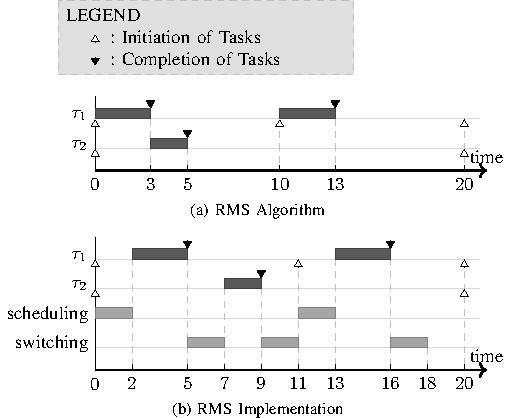
\includegraphics{rms.pdf}
\caption{A set of $2$ periodic tasks scheduled under RMS algorithm and
  the implementation, respectively. $T=T_1=10$, $T_2=20$, $C_1=3$,
  $C_2=2$. In~(b), we assume both scheduling time and switching time
  are $2$.}
\label{f:example}
\end{figure}

In this section, we introduce first how we model the states--the
static aspect--of the system using terms of given sorts, or called
data types, then how we specify the essential behaviors--the dynamic
aspect--using rewrite rules. In particular, modeling of
\emph{instantaneous behaviors} would be explained in
Sections~\ref{ss:ir}, \ref{ss:init} and~\ref{ss:inthandling}, followed
by \emph{timed behaviors} in Section~\ref{ss:timedbehavior}.

\subsection{Basic Data Types}
In our model, tasks are identified by their indexes of sort \verb|Nat|
in the $taskList$. We define a sort \verb|MaybeNat| wrapping
\verb|Nat|s to refer to some task, with \emph{constructor} \verb|some|
followed by a \verb|Nat| $n$ indicating the task indexed $n$, and
\verb|none| for no task:
\begin{verbatim}
  op none : -> MaybeNat [ctor] .
  op some_ : Nat -> MaybeNat [ctor] .
\end{verbatim}
where the keyword \verb|ctor| denotes the corresponding function
symbol to be a constructor.

A sort \verb|Stack| is introduced to model the stack of the system,
storing the tasks that are being interrupted, and equipped with
operations \verb|push|, \verb|pop| and \verb|peek| on it.
\hide{
\begin{verbatim}
  op bottom : -> Stack [ctor] .
  op _#_ : Nat Stack -> Stack [ctor] .
\end{verbatim}
}

We also need
%a sort \verb|Interval| to denote computation requirements of tasks, and 
a sort \verb|Counter| to record the execution of tasks.  We call
\emph{execution time} the time how long a task has been executing
for. A \verb|Counter| records the execution time and the computation
requirement of a task.
\hide{
\begin{verbatim}
  op [_/_] : Time Time -> Counter [ctor] .
\end{verbatim}
}

\hide{
At last, to make our model checkable by untimed model checking, it is
reasonable to reset the global variable $timer$ when it reaches an
upper bound while increasing (see Line~\ref{l:timer} in
Figure~\ref{a:schedule}) in the model. Then $timer$ is of sort
\verb|Timer| and the upper bound would be the least common multiple of
the periods of all tasks.}

The global variable $timer$ is reset when it reaches an upper bound
while increasing, which is not shown in detail in
Figure~\ref{a:schedule} but is reasonable. The upper bound is the
least common multiple of the periods of all tasks. A sort \verb|Timer|
is defined to model the $timer$.
\hide{
\begin{verbatim}
  op [_/_] : Nat NzNat -> Timer [ctor] .
\end{verbatim}
}

\subsection{Modeling the System States}
The system can be considered as consisting of several parts: the tasks
which are scheduled, the scheduler itself, the hardware including
registers and stacks, and the interrupt source. The scheduler,
i.e. the function $schedule()$, can be described by a single variable
$timer$. We present the models of the other parts one by one.

\subsubsection{Tasks}
Each task is abstracted from its functionality as a \verb|Counter|.
Overhead for scheduling and switching is considered in our model. They
are treated as two system tasks. Every task is modeled as an object
instance of some subclass of the base class \verb|Task|:
\begin{verbatim}
  class Task | cnt : Counter .
  op error : -> Object [ctor] .
\end{verbatim}
where \verb|error| is an object indicating some task that misses its
deadline.

A periodic task, which needs to be scheduled, is an object instance of
the subclass \verb|PTask| of \verb|Task| with additional attributes
\verb|priority|, \verb|period| and \verb|status|:
%  class PTask | priority : Nat, period : NzNat, 
\begin{verbatim}
  class PTask | priority : Nat, period : Nat, 
                status : Status .
  subclass PTask < Task .
\end{verbatim}
where \verb|Status| is a sort with four constant constructors
\verb|RUNNING|, \verb|INTERRUPT|, \verb|READY| and \verb|DORMANT|,
same as in the implementation.
\hide{
\begin{verbatim}
  ops RUNNING INTERRUPT READY DORMANT 
        : -> Status [ctor] .
\end{verbatim}
} 

The list of periodic tasks, the variable $taskList$ in the
implementation, is modeled as an instance of sort \verb|TaskList|,
which is a list of \verb|PTask|s and/or \verb|error|s.
\hide{
\begin{verbatim}
  op null : -> TaskList [ctor] .
  op _::_ : Object TaskList 
              ~> TaskList [ctor] .
  mb (< O:Oid : PTask |> :: L:TaskList) 
       : TaskList .
  mb (error :: L:TaskList) : TaskList .
\end{verbatim}
}
Periodic tasks are identified by their indexes in the list.

On the other hand, a system task is an object instance of the subclass
\verb|SysTask| of \verb|Task| with no extra attributes:
\begin{verbatim}
  class SysTask | .  
  subclass SysTask < Task .
\end{verbatim}
Different from periodic tasks, system tasks are organized in a
multiset of sort \verb|SysTasks|, and identified by their \verb|Oid|s.
%We abstract here from the detailed definitions thanks to the
%similarity.

\subsubsection{Hardware}
Our model considers two parts of hardware related to the interrupt
handling mechanism: the registers and the stack.

The set of registers is modeled as an object instance of the class
\verb|Regs|, with attributes \verb|pc| denoting the program counter,
\verb|mask| for the interrupt mask bit and \verb|ir| for the interrupt
request bit, respectively:
\begin{verbatim}
  class Regs | pc : TaskID, 
               mask : Bool, ir : Bool .
\end{verbatim}
where the sort \verb|TaskID| contains subsorts \verb|MaybeNat| and
\verb|Oid|, referring to some task.
\hide{
\begin{verbatim}
  subsorts MaybeNat Oid < TaskID .
\end{verbatim}
}
Some operations, such as \verb|getPc| and \verb|setMask|, are defined
on the class \verb|Regs|.

Then the hardware is described by the sort \verb|Hardware| consisting
of an instance of \verb|Regs| and a term of sort \verb|Stack|.  
\hide{
\begin{verbatim}
  op [_;_] : Object Stack ~> Hardware [ctor] .
  mb ([ < O:Oid : Regs |> ; S:Stack ]) 
       : Hardware .
\end{verbatim}
}

\subsubsection{Interrupt Source}
The interrupt source is modeled as an object of class \verb|IntSrc|,
with attributes \verb|cycle| denoting the interrupt cycle $T$, and
\verb|val| for the value which will decrease from $T$ to $0$ while
time advances:
\begin{verbatim}
  class IntSrc | val : Time, cycle : Time .
\end{verbatim}

\subsubsection{System}
The entire system in our model is a composition of the parts
introduced above, of a sort \verb|System|\footnote{Following the Maude
  convention, variables would be written in capital letters. Some
  variable declarations are not shown for simplicity.}:
\begin{verbatim}
  op _____ : TaskList Timer SysTasks 
             Hardware Object ~> System [ctor] .
  mb (L T STS HW < O : IntSrc |>) : System .
\end{verbatim}
where ``\verb|~>|'' means that the function defined is a partial
function and the keyword \verb|mb| declares a membership axiom,
stating here that a term composed of a \verb|TaskList|, a
\verb|Timer|, a \verb|SysTasks|, a \verb|Hardware| and an object
instance of class \verb|IntSrc| is of sort \verb|System|.

\subsection{Interrupt Requests}
\label{ss:ir}
Interrupt requests are performed by the source exactly every cycle
$T$, when the attribute \verb|val| decreases to \verb|zero|. The
requesting is an instantaneous action, thus is modeled by the
following instantaneous conditional rule applied on \verb|System|:
\begin{verbatim}
  crl [interrupt-request] :
    (L T STS HW ISRC) 
    => (L T STS (HW).intReq reset(ISRC))
    if (ISRC).timeout .
\end{verbatim}
where the function \verb|_.timeout| examines whether the attribute
\verb|val| equals \verb|zero|, and \verb|_.intReq| sets the \verb|ir|
bit indicating there exists an interrupt request to be handled.
\hide{
\begin{verbatim}
  op _.intReq : Hardware -> Hardware .
  eq [ REGS ; S ].intReq 
       = [ (REGS).setIr ; S ] .
\end{verbatim}
}

Then the request will wait to be handled, which is explained in
Section~\ref{ss:inthandling}.

\subsection{Task Initiation}
\label{ss:init}
Periodic tasks are initiated sequentially by the function
$updateStatus()$ in Figure~\ref{a:schedule}, which is treated as an
instantaneous action in our model. It is modeled by a recursive
function \verb|updateStatus_with_|:
\begin{verbatim}
  op updateStatus_with_ : TaskList Timer 
                            -> TaskList . 
\end{verbatim}
%  eq updateStatus null with TIMER = null .
%  eq updateStatus (TASK :: L) with TIMER
%     = (update TASK with TIMER) 
%       :: (updateStatus L with TIMER) .
which applies function \verb|update_with_| on individual task
sequentially to update the status
(Lines~\ref{l:startupdate}-\ref{l:endupdate} in
Figure~\ref{a:schedule}):
\begin{verbatim}
  op update_with_ : Object Timer ~> Object .
  ceq update < O : PTask | period : T, 
                           status : ST > 
        with TIMER
      = if ST == DORMANT 
        then < O : PTask | status : READY >
        else error fi
      if TIMER rem T == 0 .
  eq update < O : PTask | status : ST > 
       with TIMER
     = if ST == RUNNING 
       then < O : PTask | status : INTERRUPT >
       else < O : PTask |> fi [otherwise] .
\end{verbatim}
with \verb|TIMER| the current value of the global variable $timer$.
Given a task, if \verb|TIMER|($timer$) can be divided by its period
\verb|T|, this task should be initiated.  In the case where the task
should be initiated, it is set \verb|READY| if its \verb|status| is
\verb|DORMANT|; otherwise that means the previous job of this task is
not complete, hence it misses its deadline, producing an
\verb|error|. In the other case where the task should not be
initiated, its \verb|status| changes only if it is \verb|RUNNING|.

We can see that \verb|updateStatus_with_| behaves the same as
$updateStatus()$ in Figure~\ref{a:schedule}.

\subsection{Interrupt Handling and Task Scheduling}
\label{ss:inthandling}
When an interrupt request occurs, it may not be detected immediately
by the system. It requires the bit \verb|mask| to be cleared. Once the
request is detected, it is handled in two steps: the interrupt
handling mechanism of the hardware (such as clearing \verb|ir|,
pushing context into stack and so on), and to invoke the function
$schedule()$. This behavior is modeled by the following instantaneous
rewrite rule:
\begin{verbatim}
  crl [interrupt-handle] :
    SYSTEM 
    => ((SYSTEM).interrupt).startScheduling
    if (SYSTEM).existInt .
\end{verbatim}
where \verb|_.existInt| checks whether \verb|mask| is cleared
\emph{and} \verb|ir| is set. The function \verb|_.interrupt| models
the interrupt handling mechanism performed by the hardware and does
four things: (i) clearing the bit \verb|ir|, which means the request
has been handled; (ii) pushing the current \verb|pc| into the stack,
storing the interrupted context; (iii) assigning \verb|scheduling| of
sort \verb|Oid| to \verb|pc|, which indicates that the system is
scheduling; and (iv) setting the bit \verb|mask|, to mask coming
interrupt requests.

Unlike periodic tasks, even though the scheduling stage is modeled by
a \verb|Counter|, its functionality is too important to be abandoned.
We divide the behaviors of scheduling into three parts.  The first
part contains its timed behaviors. This part is modeled by regarding
scheduling as a system task of sort \verb|SysTask|. Modeling timed
behaviors of tasks is explained in Section~\ref{ss:timedbehavior}.
The other two parts together define its functionality. The second part
corresponds to Lines~\ref{l:updatestatus}-\ref{l:inc} in
Figure~\ref{a:schedule}. It updates the status of $taskList$ and
increases $timer$ by $1$. This part is modeled by function
\verb|_.startScheduling| which applies instantaneously at the
beginning of scheduling, as shown in rule \verb|interrupt-handle|:
\begin{verbatim}
  op _.startScheduling : System -> System .
  eq (L T STS HW ISRC).startScheduling 
     = ((updateStatus L with T) 
        inc(T) STS HW ISRC) .
\end{verbatim}
The third part corresponds to
Lines~\ref{l:startrun1st}-\ref{l:endrun1st}, searching the first
should-be-run periodic task and setting it to execute. It is modeled
by function \verb|_.finishScheduling|, which applies instantaneously
at the end of scheduling:
\begin{verbatim}
  op _.finishScheduling : System -> System .
  eq (L T STS HW ISRC).finishScheduling
     = (L T (finish scheduling in STS) 
        HW ISRC).run1stTask .
\end{verbatim}
where \verb|finish_in_| resets the counter of task \verb|scheduling|,
and \verb|_.run1stTask| models
Lines~\ref{l:startrun1st}-\ref{l:endrun1st} in
Figure~\ref{a:schedule}, searching the task with highest priority
that has status \verb|INTERRUPT| or \verb|READY| then performing an
\emph{interrupt return} or executing it, respectively.

When the execution time of the system task \verb|scheduling| reaches
its computation requirement, scheduling is finished. We model this
instantaneous action with the following rule:
\begin{verbatim}
  crl [scheduling-finish] :
    (L T STS HW ISRC) 
    => (SYSTEM).finishScheduling
    if SYSTEM := (L T STS HW ISRC) 
       /\ (SYSTEM).running == scheduling 
       /\ scheduling isComplete?in STS .
\end{verbatim}
where function \verb|_.running| returns the current \verb|pc| value of
the system, and \verb|_isComplete?in_| checks whether the execution
time of the task reaches its computation requirement.  
\hide{
\begin{verbatim}
  op _mayFinish?in_ : Oid SysTasks ~> Bool .
  eq O mayFinish?in [ < O : SysTask | cnt : C > REST ] 
       = C mayFinish? .
  op _mayFinish? : Counter -> Bool .
  eq [ R / [ MIN , MAX ] ] mayFinish?
       = if R lt MIN then false else true fi .
\end{verbatim}}

Similar to scheduling, the switching stage is also divided into timed
behaviors of \verb|switching| and its functionality. \verb|switching|
starts when the running periodic task is complete, and finishes when
itself is so. Two similar instantaneous rules \verb|switching-start|
and \verb|switching-finish| are defined to model the functionality of
switching. 
\hide{
\begin{verbatim}
  crl [task-finish] :
    (L T STS HW ISRC) 
    => (SYSTEM).startSwitching
    if SYSTEM := (L T STS HW ISRC)
       /\ some N := (SYSTEM).running
       /\ some N isComplete?in L .
  crl [switching-finish] :
    (L T STS HW ISRC) 
    => (SYSTEM).finishSwitching
    if SYSTEM := (L T STS HW ISRC)
       /\ (SYSTEM).running == switching
       /\ switching isComplete?in STS .
\end{verbatim}
}

\subsection{Timed Behaviors of the System}
\label{ss:timedbehavior}
Timed behaviors of the system consist of two parts: the execution of
tasks and the execution of the interrupt source. Both are modeled
together by the following single \emph{standard} tick
rule\footnote{The keyword \texttt{nonexec} should be given to allow
  the Real-Time Maude engine to apply the rule with some
  strategies.}~\cite{DBLP:journals/entcs/OlveczkyM07a}:
\begin{verbatim}
  crl [tick]:
    {SYSTEM} => {delta(SYSTEM, R)} in time R 
    if R le mte(SYSTEM) [nonexec] .
\end{verbatim}
where \verb|delta| defines the effects of time elapse on the system,
and \verb|mte| denotes the \emph{m}aximum amount of \emph{t}ime
allowed to \emph{e}lapse from the current state until an instantaneous
transition \emph{must} be performed. In fact, the core to model timed
behaviors is to define functions \verb|delta| and \verb|mte|. Notice
that the variable \verb|R| is \emph{continuous} with respect to the
specific time domain\footnote{Real-Time Maude contains built-in
  modules to define the time domain to be natural numbers and rational
  numbers, specifying \emph{discrete} time domains and \emph{dense}
  time domains, respectively.}  that we choose to instantiate our
model on, which is different from timed automata that discretize dense
time by defining ``clock region''.

Time affects the system by advancing both the running task whose $ID$
is loaded at \verb|pc| and the interrupt source simultaneously.  While
time elapses, \verb|cnt| of the former increases and \verb|val| of the
latter decreases, respectively:
\begin{verbatim}
  ceq delta((L T STS HW ISRC), R)
      = (deltaTask(ID, L, R) 
         T STS HW (deltaIS(ISRC, R)))
      if ID := (HW).getPc /\ ID :: MaybeNat .
\end{verbatim}
where the last condition states that \verb|ID| is of sort
\verb|MaybeNat|. Due to similarity, we omit details for the case where
\verb|ID| is of sort \verb|Oid| and \verb|deltaTask| applies on
\verb|STS| instead of \verb|L|.

\verb|mte|, the maximum amount of time allowed to elapse, depends on
when the next instantaneous action must perform. Therefore, it is
decided by three arguments: the remaining time to complete the running
task, the remaining time to request the next interrupt, and whether or
not there exists an interrupt request detected for the moment:
\begin{verbatim}
  ceq mte(L T STS HW ISRC)
      = minimum(mteTask(ID, L),
                mteIS(ISRC), mteIr(HW))
      if ID := (HW).getPc /\ ID :: MaybeNat .
\end{verbatim}
where \verb|mteIr| returns \verb|zero| if there exists an interrupt
request detected in the system, or \verb|INF| which represents
\emph{infinity} otherwise. Again we do not show the case where
\verb|ID| is of sort \verb|Oid|, which is very similar. 
\hide{
We should
point out that \verb|mteTask| computes the remaining time to reach the
maximum of the computation requirement of the task, since that is the
time at which a \verb|task-finish| transition \emph{must} happen.
}


\section{Formal Verification}
\label{s:verification}
In this section, we analyze our model of the RMS implementation within
different realistic scenarios.  Notice that from any (reasonable)
given initial state, the number of reachable states is finite, but may
be unknown, thanks to the upper bound given to $timer$, which provides
the potential for applying the untimed model checker.

\subsection{Properties}
We consider two properties in this paper: schedulability and
correctness. By schedulability, we examine whether a given task set is
schedulable by the implementation. By correctness, we verify whether
the implementation schedules periodic tasks exactly with respect to
the RMS algorithm.

To verify the schedulability of a given set of periodic tasks, we
define an atomic proposition \verb|taskTimeout| to hold if there
exists an \verb|error| in $taskList$ of the current state, that is,
some task misses its deadline:
\begin{verbatim}
  op taskTimeout : -> Prop [ctor] .
  eq {L T STS HW ISRC} |= taskTimeout 
     = containError(L) .
\end{verbatim}
where \verb|containError| returns \verb|true| if there is an
\verb|error| existing in \verb|L|. Then schedulability can be
formalized as the temporal logic formula: \verb|[](~taskTimeout)|,
expressing that the proposition \verb|taskTimeout| is always false. As
the property is not \emph{clock-related}, given an initial state
\verb|init|, the following untimed model checking command returns
\verb|true| if the schedulability property holds with no time limit;
otherwise a trace showing a counterexample is provided:
\begin{verbatim}
  (mc init |=u [](~taskTimeout) .)
\end{verbatim}

Another important objective is to verify the correctness of the
implementation.  The atomic proposition \verb|correct| is hence
defined to hold if the running periodic task is the one requested to
be executed with the highest priority:
\begin{verbatim}
  op correct : -> Prop [ctor] .
  ceq {L T STS HW ISRC} |= correct
      = if ID :: MaybeNat then shouldRun(ID, L)
        else true fi
      if ID := (HW).getPc .
\end{verbatim}
where \verb|shouldRun(ID, L)| returns \verb|true| if the task
identified by \verb|ID|, probably \verb|none|, is the one possessing
the highest priority among those whose status is not
\verb|DORMANT|. Note that during verification, we do not care the
behaviors after some task misses its deadline. Therefore, the
correctness property is formalized by the temporal logic formula:
\verb|([]correct)\/(correct U taskTimeout)|, stating that
\verb|correct| is always true, or is true until \verb|taskTimeout|
holds. It can be verified by the following untimed model checking
command provided an initial state \verb|init|:
\begin{verbatim}
  (mc init |=u ([]correct) 
               \/ (correct U taskTimeout) .)
\end{verbatim}

\subsection{Scenarios}
\label{ss:results}
We use the following setting for our verification, which is from the 
statistics provided by our industrial partner:
\begin{itemize}
\item The interrupt cycle $T$ is $5ms$.
\item The scheduling time is $38{\mu}s$ and the switching time is
  $20{\mu}s$.  
\hide{\item The scheduling time ranges from $5{\mu}s$
  to $9{\mu}s$, and the switching time ranges from $2{\mu}s$ to
  $4{\mu}s$.}
\item The initial state is with empty stack, empty \verb|pc|, cleared 
\verb|mask| and cleared \verb|ir|.
\end{itemize}

We have analyzed our model in ten different scenarios, including both
realistic ones provided by our industrial partner and experimental
ones designed by ourselves, four of them are described below:
\begin{itemize}
\item Scenario~(i) with two tasks $\tau_1$ and $\tau_2$: $T_1=5ms$,
  $C_1=3ms$, $T_2=25ms$ and $C_2=7ms$.
\item Scenario~(ii) with two tasks $\tau_1$ and $\tau_2$: $T_1=5ms$,
  $C_1=2ms$, $T_2=25ms$ and $C_2=2.3ms$.
\item Scenario~(iii) with three tasks $\tau_1$, $\tau_2$ and $\tau_3$:
  $T_1=5ms$, $C_1=2.7ms$, $T_2=10ms$, $C_2=2ms$, $T_3=25ms$ and
  $C_3=3ms$.
\item Scenario~(iv) with three tasks $\tau_1$, $\tau_2$ and $\tau_3$:
  $T_1=5ms$, $C_1=2.5ms$, $T_2=10ms$, $C_2=1.5ms$, $T_3=15ms$ and
$C_3=4.5ms$.
\end{itemize}
Note that thanks to the powerful expressiveness of Real-Time Maude, we
only need to define an initial state of sort \verb|System| to specify
a given task set. No necessity to modify the model is needed.

\hide{
\begin{itemize}
\item Scenario (i) with two tasks: one having period $5ms$ and
  computation requirement $[2.4ms, 3ms]$, and the other having period
  $25ms$ and computation requirement $[6.1ms, 7ms]$.
\item Scenario (ii) with two tasks: one having period $5ms$ and
  computation requirement $[1.8ms, 2ms]$, and the other having period
  $25ms$ and computation requirement $[2.1ms, 2.3ms]$.
\item Scenario (iii) with three tasks: the first having period $5ms$
  and computation requirement $[2.5ms, 2.7ms]$, the second having
  period $10ms$ and computation requirement $[1.5ms, 2ms]$, and the
  third having period $25ms$ and computation requirement $[2.6ms,
    3ms]$.
\item Scenario (iv) with three tasks: the first having period $5ms$
  and computation requirement $[2.2ms, 2.5ms]$, the second having
  period $10ms$ and computation requirement $[1.4ms, 1.5ms]$, and the
  third having period $15ms$ and computation requirement $[4.3ms,
    4.5ms]$.
\end{itemize}
}


\begin{figure*}[!t]
\centering
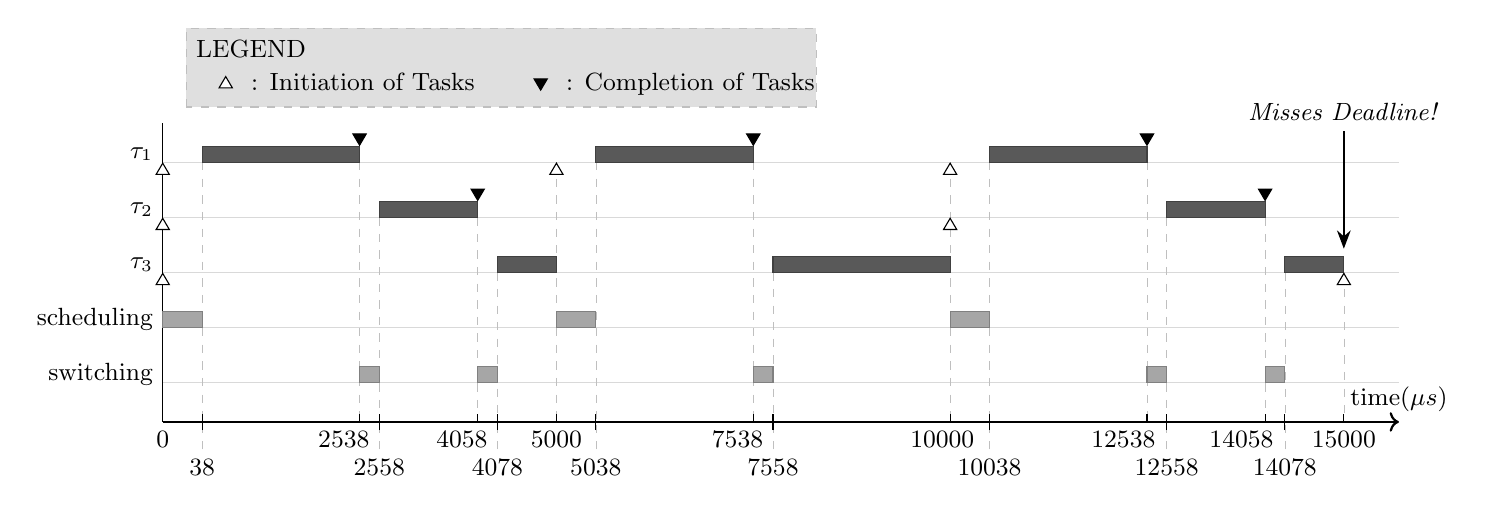
\begin{tikzpicture}[font=\small,
    % styles
    system task/.style={fill=gray!70,draw=gray},
    periodic task/.style={fill=gray!70!black,draw=gray!50!black},
    task line/.style={gray!30,very thin},
    time line/.style={gray!50,very thin,dashed},
    short line/.style={gray!50,very thin,dashed},
    init/.style={{Triangle[fill=white,scale=1.3]}-},
    complete/.style={{Triangle[scale=1.3]}-}]

  % grid
  \foreach \x in {0.5,1.2,...,3.3}
    \draw[task line] (0,\x) -- (15.7,\x);

  % time indicator
  \draw (0,0) node [below] {$0$};
  \draw[time line] (0.5,3.3) -- (0.5,0);
  \draw (0.5,-0.35) node [below] {$38$} [short line] -- +(0,0.35);
  \draw (0.5,-3pt) -- (0.5,3pt);
  \draw[time line] (2.5,3.3) -- (2.5,0);
  \draw (2.3,0) node [below] {$2538$};
  \draw (2.5,0) -- (2.5,3pt);
  \draw[time line] (2.75,2.6) -- (2.75,0);
  \draw (2.75,-0.35) node [below] {$2558$} [short line] -- +(0,0.35);
  \draw (2.75,-3pt) -- (2.75,3pt);
  \draw[time line] (4,2.6) -- (4,0);
  \draw (3.8,0) node [below] {$4058$};
  \draw (4,0) -- (4,3pt);
  \draw[time line] (4.25,1.9) -- (4.25,0);
  \draw (4.25,-0.35) node [below] {$4078$} [short line] -- +(0,0.35);
  \draw (4.25,-3pt) -- (4.25,3pt);

  \draw[time line] (5,3.3) -- (5,0);
  \draw (5,0) node [below] {$5000$};
  \draw (5,0) -- (5,3pt);
  \draw[time line] (5.5,3.3) -- (5.5,0);
  \draw (5.5,-0.35) node [below] {$5038$} [short line] -- +(0,0.35);
  \draw (5.5,-3pt) -- (5.5,3pt);
  \draw[time line] (7.5,3.3) -- (7.5,0);
  \draw (7.3,0) node [below] {$7538$};
  \draw (7.5,0) -- (7.5,3pt);
  \draw[time line] (7.75,1.9) -- (7.75,0);
  \draw (7.75,-0.35) node [below] {$7558$} [short line] -- +(0,0.35);
  \draw (7.75,-3pt) -- (7.75,3pt);

  \draw[time line] (10,3.3) -- (10,0);
  \draw (9.9,0) node [below] {$10000$};
  \draw (10,0) -- (10,3pt);
  \draw[time line] (10.5,3.3) -- (10.5,0);
  \draw (10.5,-0.35) node [below] {$10038$} [short line] -- +(0,0.35);
  \draw (10.5,-3pt) -- (10.5,3pt);
  \draw[time line] (12.5,3.3) -- (12.5,0);
  \draw (12.2,0) node [below] {$12538$};
  \draw (12.5,0) -- (12.5,3pt);
  \draw[time line] (12.75,2.6) -- (12.75,0);
  \draw (12.75,-0.35) node [below] {$12558$} [short line] -- +(0,0.35);
  \draw (12.75,-3pt) -- (12.75,3pt);
  \draw[time line] (14,2.6) -- (14,0);
  \draw (13.7,0) node [below] {$14058$};
  \draw (14,0) -- (14,3pt);
  \draw[time line] (14.25,1.9) -- (14.25,0);
  \draw (14.25,-0.35) node [below] {$14078$} [short line] -- +(0,0.35);
  \draw (14.25,-3pt) -- (14.25,3pt);
  \draw[time line] (15,1.9) -- (15,0);
  \draw (15,0) node [below] {$15000$};
  \draw (15,0) -- (15,3pt);

  % axes
  \draw[->,thick] (0,0) -- (15.7,0) node [above] {time(${\mu}s$)};
  \draw[thin] (0,0) -- (0,3.8);

  % tips of tasks
  \draw (0,0.6) node [left] {switching};
  \draw (0,1.3) node [left] {scheduling};
  \draw (0,2) node [left] {$\tau_3$};
  \draw (0,2.7) node [left] {$\tau_2$};
  \draw (0,3.4) node [left] {$\tau_1$};

  % tasks
  \filldraw[system task] (0,1.2) rectangle +(0.5,0.2);
  \filldraw[periodic task] (0.5,3.3) rectangle +(2,0.2);
  \filldraw[system task] (2.5,0.5) rectangle +(0.25,0.2);
  \filldraw[periodic task] (2.75,2.6) rectangle +(1.25,0.2);
  \filldraw[system task] (4,0.5) rectangle +(0.25,0.2);
  \filldraw[periodic task] (4.25,1.9) rectangle +(0.75,0.2);
  
  \filldraw[system task] (5,1.2) rectangle +(0.5,0.2);
  \filldraw[periodic task] (5.5,3.3) rectangle +(2,0.2);
  \filldraw[system task] (7.5,0.5) rectangle +(0.25,0.2);
  \filldraw[periodic task] (7.75,1.9) rectangle +(2.25,0.2);
  
  \filldraw[system task] (10,1.2) rectangle +(0.5,0.2);
  \filldraw[periodic task] (10.5,3.3) rectangle +(2,0.2);
  \filldraw[system task] (12.5,0.5) rectangle +(0.25,0.2);
  \filldraw[periodic task] (12.75,2.6) rectangle +(1.25,0.2);
  \filldraw[system task] (14,0.5) rectangle +(0.25,0.2);
  \filldraw[periodic task] (14.25,1.9) rectangle +(0.75,0.2);

  % initiation of tasks
  \foreach \x in {0,5,10}
    \draw [init] (\x,3.3) -- +(0,-0.1);
  \foreach \x in {0,10}
    \draw [init] (\x,2.6) -- +(0,-0.1);  
  \foreach \x in {0,15}
    \draw [init] (\x,1.9) -- +(0,-0.1); 

  % completion of tasks
  \draw [complete] (2.5,3.5) -- +(0,0.1);
  \draw [complete] (4,2.8) -- +(0,0.1);
  \draw [complete] (7.5,3.5) -- +(0,0.1);
  \draw [complete] (12.5,3.5) -- +(0,0.1);
  \draw [complete] (14,2.8) -- +(0,0.1);

  % text
  \draw[{Stealth}-,thick] (15,2.2) -- +(0,1.5)
    node [above] {\emph{Misses Deadline!}};

  % legend
  \begin{scope}[xshift = -1.2cm]  
    \draw [fill=gray!25,draw=gray!50,dashed] (1.5,4) rectangle +(8,1);
    \draw (1.5,4.5) node [above right] {LEGEND};
    \draw [init] (2,4.4) -- +(0,-0.1);
    \draw (2.2,4.55) node [below right] {: Initiation of Tasks};
    \draw [complete] (6,4.2) -- +(0,0.1);
    \draw (6.2,4.55) node [below right] {: Completion of Tasks};
  \end{scope}
\end{tikzpicture}
\caption{A counterexample of schedulability in Scenario~(iv). The first
  job instance of $\tau_3$ misses its deadline at time $15ms$, which
  is the initiation time for the second job instance of $\tau_3$.}
\label{f:counterexample}
\end{figure*}

Instantiating our model on dense time domain and choosing the
\emph{maximal time sampling strategy}, the results of the model
checking show that the correctness property holds in all scenarios. As
to the schedulability property, it holds in Scenarios~(i-iii), but
fails in Scenario~(iv).  One counterexample of the schedulability
within Scenario~(iv), returned by the model checking command, is
pictured in Figure~\ref{f:counterexample}, where the third task
$\tau_3$ misses its deadline at the time $15ms$.

The results above have demonstrated that our approach is capable of
handling realistic industrial systems. However to further exam the
efficiency of our approach, we also apply our method to larger test
scenarios. Test scenarios are generated randomly. We verify the
schedulability of them under the above setting on an Intel Core 2 Quad
Q9550, 2.83GHz, 4-cores machine with 8GB RAM running 64-bit Ubuntu
15.04. Among the 50 generated test scenarios with 5 tasks, we find
that the execution time of the model checking command for each
scenario varies from about $300ms$ up to a timeout, which is set to
$90$ minutes. This is because the efficiency of model checking depends
on the scale of the state space. And the scale is further positively
correlated with $mn$, where $m$ is the upper bound of $timer$ and $n$
is the number of periodic tasks. By the generated test scenarios, it
turns out that the model checking command for schedulability in our
model is able to handle scenarios, where $mn$ is up to about $10^6$,
in an acceptable period of time say $90$ minutes.


\subsection{Evaluation}
We now show in this section that our results are both sound and
complete.

An analysis method is called \emph{sound} if any counterexample found
using such a method is a real counterexample of the question, and
\emph{complete} if the fact that no counterexample can be found using
such a method implies no counterexample exists for the question in
analysis. The soundness of our results is trivial to check, simply by
examining the counterexamples found. For instance, the counterexample
shown in Figure~\ref{f:counterexample} is a real counterexample,
implying that the result for schedulability of Scenario~(iv) is
sound. But this is not the case for completeness, since we choose
instantiating our model on dense time domain to make it more real but
giving rise to an infinite state space which is unfeasible to exhaust.

In general, completeness of untimed model checking cannot be achieved
for any systems, any time sampling strategies and any
properties. However, \"Olveczky and Meseguer proved the completeness
of untimed temporal logic model checking, under the maximal time
sampling strategy, for a large class of real-time systems possessing a
set of ``good'' properties that is called \emph{time-robustness}, and
for a set of ``good'' LTL formulae constructed by
\emph{tick-invariant} propositions\footnote{We avoid introducing the
  definitions of time-robustness and tick-invariance, due to the
  requirements of extra rewriting logic
  background.}~\cite{DBLP:journals/entcs/OlveczkyM07a}:
\begin{theorem}[\cite{DBLP:journals/entcs/OlveczkyM07a}]
\label{t:completeness}
Given a time-robust real-time rewrite theory $\cal R$, a set $AP$ of
tick-invariant atomic propositions, an LTL formula $\Phi$ (excluding
the \emph{next} operator $\bigcirc$) whose atomic propositions are
contained in $AP$. The untimed temporal logic model checking verifying
$\Phi$ is \emph{complete} under the maximal time sampling strategy.
\end{theorem}

Therefore, we achieve the following theorem, showing that the results
in Section~\ref{ss:results} are complete.
\begin{theorem}
\label{t:main}
Our approach using untimed model checking to verify the schedulability
and the correctness of our model is complete.
\end{theorem}
\begin{IEEEproof}
By showing that our model is time-robust and that the two defined
atomic propositions--\verb|taskTimeout| and \verb|correct|--are
tick-invariant, then using Theorem~\ref{t:completeness}. For a more
detailed proof, see the Appendix.
\end{IEEEproof}


\section{Related Work}
\label{s:relate}
In this section we discuss our results with related
work in three directions.

Considering schedulability test, Liu and
Layland~\cite{DBLP:journals/jacm/LiuL73} gave the famous sufficient
condition that a set of periodic tasks is schedulable with respect to
RMS if $\displaystyle \Sigma^n_{i=1} C_i/T_i \le n(2^{1/n}-1)$
holds. Then a more sufficient condition, known as \emph{Hyperbolic
  Bound}, which has the same complexity as Liu and Layland's, was
proposed in~\cite{DBLP:journals/tc/BiniBB03}. On the other hand,
necessary and sufficient conditions for schedulability were derived
independently in~\cite{DBLP:journals/rts/SpruntSL89}
and~\cite{audsley1993deadline}, requiring more sophisticated analysis
on the task set. Nevertheless, all these results take no overhead into
account, being not as realistic as ours. Katcher et al. did consider
overhead in their schedulability analysis, under several models based
on different kinds of popular
implementations~\cite{DBLP:journals/tse/KatcherAS93}.  However, our
target implementation is not in their scope. Furthermore, compared
with those theoretical analyses, our approach based on formal modeling
and verification has three advantages. One is that if our
schedulability test answers ``no'', it returns at the same time a real
counterexample, which is able to guide our engineer to adjust the
design, by changing either the priorities or even the scheduling
algorithm. The second is that, when a fresh scheduling strategy is
applied, our analysis can be adjusted only by modifying the model,
while theoretical approaches may need thorough analyses and reasoning.
The last one is that, considering overhead and details of hardware do
introduce some kind of non-determinism into the model. For example, in
our model, if the running task is complete \emph{right} at the time
when an interrupt request occurs, two different behaviors are
possible: (i) the system performs task switching, during which the
interrupt request is masked, hence the scheduling and initiation of
tasks may be delayed; (ii) the system answers the interrupt request
immediately, the switching being delayed. Tackling such
non-determinism via theoretical analyses seems more complicated than
our automatic approach.

\cite{TianD2011} and~\cite{DBLP:conf/iceccs/CuiDT14} also made use of
model checking to analyze the RMS algorithm along the same line but
with different languages and tools. The RMS algorithm is investigated
using an extension of SPIN~\cite{DBLP:journals/tse/Holzmann97}
in~\cite{TianD2011}, while the logic programming language
TMSVL~\cite{DBLP:conf/icfem/HanDW12} and its model checker are applied
in~\cite{DBLP:conf/iceccs/CuiDT14}. The work presented
in~\cite{TianD2011} and~\cite{DBLP:conf/iceccs/CuiDT14} has two main
differences with ours. The first one, which is also the motivational
one, is that they considered only the ideal setting of the algorithm
as in~\cite{DBLP:journals/jacm/LiuL73}, instead of an implementation
which contains much more complex details. In fact, our model of the
implementation can easily degenerate to a model of the RMS algorithm,
if we let the times for scheduling and switching be zero. The other
difference is that when adding a new task into the task set, the
models in~\cite{TianD2011} and~\cite{DBLP:conf/iceccs/CuiDT14} should
be modified by explicitly defining a sub-model of the new task and its
behaviors. In particular, the scheduling part of the model
in~\cite{TianD2011} needs adjustments as well to include a new
task. Nevertheless, a new task set is specified in our approach merely
by giving a new initial state, without necessity to modify the model,
as already emphasized in Section~\ref{ss:results}. On the other hand,
\cite{TianD2011} used a discrete time domain in the model, while we
employ a generic time domain, which is flexible to be instantiated on
either discrete or dense ones. In~\cite{DBLP:conf/iceccs/CuiDT14}, the
time domain is dense, and a modeling strategy like our maximal time
sampling strategy is applied to reduce the state space. However, a
completeness statement like Theorem~\ref{t:main} was not given
in~\cite{DBLP:conf/iceccs/CuiDT14}.

Finally, Maude and Real-Time Maude have been successfully applied on
large numbers of applications~\cite{DBLP:journals/jlp/Meseguer12},
especially on communication protocols, real-time and cyber-physical
systems. But few results are achieved on scheduling problems. RMS is
investigated using Real-Time Maude for the first time.


\section{Conclusion}
\label{s:conclusion}
We have formally modeled a realistic implementation of RMS using
Real-Time Maude, a modeling language based on rewriting logic. By
taking into account the overhead of scheduling and switching, and by
modeling some mechanism of the hardware, our model contains sufficient
details to be analyzed for the behaviors of the real target
system. Two important properties--schedulability and correctness--are
verified by model checking on our model, within several key
scenarios. We demonstrate the soundness and completeness of our
results.


%% \begin{figure}[!t]\centering
%% 	\includegraphics[width=8.5cm]{FIG1.eps}
%% 	\caption{Magnetization as a function of applied field. Note that ``Fig.'' is abbreviated. There is a period after the figure number, followed by two spaces. It is good practice to explain the significance of the figure in the caption.}\label{FIG_1}
%% \end{figure}


\appendix[Proof of Theorem~\ref{t:main}]
\label{a:proof}
\setcounter{theorem}{0}
\renewcommand{\thetheorem}{\thesection.\arabic{theorem}}
\newcommand{\lrps}[2]{\rightarrow^{#1}_{#2}}

We show here a detailed proof of Theorem~\ref{t:main}.

Some more preliminaries from~\cite{DBLP:journals/entcs/OlveczkyM07a}
are needed. A term $t$ is called \emph{ground} if it contains no
variables. For a set $P\subseteq AP$ of atomic propositions and ground
terms $t,t'$, we write $t\simeq_P t'$ (or $t\simeq t'$ for simplicity
when $P$ is implicit) if $t$ and $t'$ satisfy exactly the same set of
propositions from $P$.

Time-robustness is a set of properties expected from a well-behaved
real-time rewrite theory. We avoid introducing the accurate definition
of time-robustness, but instead give the following lemma to prove
time-robustness:
\begin{lemma}[\cite{DBLP:journals/entcs/OlveczkyM07a}]
\label{l:timerobustness}
Let $\cal R$ be an object-oriented specification with a standard tick
rule, and let the infinity element \verb|INF| be the only element in
the time domain which is not a normal time value.
%and let the time domain be \emph{linear}.
Then $\cal R$ is time-robust if the following conditions are satisfied
for all appropriate ground terms $t$ and $r,r'$:
\begin{enumerate}
\item
[(i)] \verb|mte(delta(|$t$\verb|,|$r$\verb|))| $=$
\verb|mte(|$t$\verb|) monus |$r$, for all $r\le$
\verb|mte(|$t$\verb|)|, where \verb|monus| is the built-in minus
operation defined on sort \verb|Time|;

\item
[(ii)] \verb|delta(|$t$\verb|,|$0$\verb|)| $= t$;

\item
[(iii)] \verb|delta(delta(|$t$\verb|,|$r$\verb|),|$r'$\verb|)| $=$
\verb|delta(|$t$\verb|,|$r+r'$\verb|)|, for $r+r'\le$
\verb|mte(|$t$\verb|)|;

\item
[(iv)] \verb|mte(|$\sigma(l)$\verb|)|$= 0$ for each ground instance
$\sigma(l)$ of each left-hand side of an instantaneous rewrite rule.
\end{enumerate}
\end{lemma}

Each one-step rewrite can be categorized and then tick-invariance can
be defined:
\begin{definition}[\cite{DBLP:journals/entcs/OlveczkyM07a}]
A one-step rewrite $t\lrps{r}{1}t'$ using a tick rule and having
duration $r$ is:\\
- a \emph{maximal tick step}, written $t\lrps{r}{max}t'$, if there is
no time value $r'>r$ such that $t\lrps{r'}{1}t''$ for some $t''$; \\
- an \emph{$\infty$ tick step}, written $t\lrps{r}{\infty}t'$, if
for each time value $r'>0$, there is a tick rewrite step
$t\lrps{r'}{1}t''$; and \\
- a \emph{non-maximal tick step} if there is a maximal tick step
$t\lrps{r'}{max}t''$ for $r'>r$.
\end{definition}
\begin{definition}[\cite{DBLP:journals/entcs/OlveczkyM07a}]
  A time-robust specification $\cal R$ is \emph{tick-invariant} with
  respect to a set $P$ of propositions if and only if it is the case
  that $t\simeq_P t'$ holds for each non-maximal or $\infty$ tick step
  $t\lrps{r}{}t'$.
\end{definition}

The following lemma is needed to prove the tick-invariance of our
defined propositions:
\begin{lemma}[\cite{DBLP:journals/entcs/OlveczkyM07a}]
\label{l:tickinv}
Let $\cal R$ be a time-robust object-oriented specification with a
standard tick rule, and let the infinity element \verb|INF| be the
only element in the time domain which is not a normal time value.
%and let the time domain be \emph{linear}. 
Then $\cal R$ is tick-invariant with respect to a set $P$ of atomic
propositions if \verb|{|$t$\verb|}| $\simeq_P$
\verb|{delta(|$t$\verb|,|$r$\verb|)}| for all $t,r$ with $r<$
\verb|mte(|$t$\verb|)|.
\end{lemma}

\newcommand{\mteTask}[2]{\texttt{mteTask(}#1\texttt{,}#2\texttt{)}}
\newcommand{\deltaTask}[3]{\texttt{deltaTask(}#1\texttt{,}#2\texttt{,}#3\texttt{)}}
\newcommand{\mteIS}[1]{\texttt{mteIS(}#1\texttt{)}}
\newcommand{\deltaIS}[2]{\texttt{deltaIS(}#1\texttt{,}#2\texttt{)}}
\newcommand{\IntSrc}[3]{\texttt{<}#1\texttt{:IntSrc|val:}#2\texttt{,cycle:}#3\texttt{>}}
\newcommand{\mteIr}[1]{\texttt{mteIr(}#1\texttt{)}}
\newcommand{\mteS}[1]{\texttt{mte(}#1\texttt{)}}
\newcommand{\deltaS}[2]{\texttt{delta(}#1\texttt{,}#2\texttt{)}}
 
Several auxiliary lemmas are proved:
\begin{lemma}
\label{l:auxtask}
Given $ID$ of sort \verb|MaybeNat| and $L$ of sort \verb|TaskList|,
\verb|mteTask(|$ID$\verb|,deltaTask(|$ID$\verb|,|$L$\verb|,|$r$\verb|))|
$=$ \verb|mteTask(|$ID$\verb|,|$L$\verb|)| \verb|monus| $r$ for all
$r\le$ \verb|mteTask(|$ID$\verb|,|$L$\verb|)|.
\end{lemma}
\begin{IEEEproof}
If $ID=$ \verb|none|, the case is trivial. By definition,
\verb|mteTask(none,deltaTask(none,|$L$\verb|,|$r$\verb|))| $=$
\verb|mteTask(none,|$L$\verb|)| $=$ \verb|INF| $=$
\verb|mteTask(none,|$L$\verb|)| \verb|monus| $r$. Otherwise, $ID=$
\verb|some| $N$ with $N$ of sort \verb|Nat|. Assume that the
\verb|cnt| of the $N$th task in $L$ is
\verb|[|$r_e$\verb|/|$C$\verb|]|. Then by definition,
\verb|deltaTask(|$ID$\verb|,|$L$\verb|,|$r$\verb|)| $= L'$, where the
$N$th task in $L'$ has \verb|cnt| value being
\verb|[|$(r_e+r)$\verb|/|$C$\verb|]|. Hence,
\begin{IEEEeqnarray*}{Cl}
  & \mteTask{ID}{\deltaTask{ID}{L}{r}}
\\  
= & \mteTask{ID}{L'}
\\
= & C~\verb|monus|~(r_e+r) 
= (C~\verb|monus|~r_e)~\verb|monus|~r 
\\
= & \mteTask{ID}{L}~\verb|monus|~r~. 
\end{IEEEeqnarray*}
\end{IEEEproof}
\begin{lemma}
\label{l:auxis}
Given $ISRC$ of class \verb|IntSrc| representing an reasonable state
of interrupt source in our model, \mteIS{\deltaIS{$ISRC$}{$r$}} $=$
\mteIS{$ISRC$} \verb|monus| $r$ for all $r\le$ \mteIS{$ISRC$}.
\end{lemma}
\begin{IEEEproof}
A reasonable $ISRC$ must be of the form \IntSrc{$O$}{$v$}{$T$} with
$v\le T$. Thus by definition, 
\begin{IEEEeqnarray*}{Cl}
  & \mteIS{\deltaIS{ISRC}{r}}
\\  
= & \mteIS{\IntSrc{O}{(v~\texttt{monus}~r)}{T}}
\\
= & v~\verb|monus|~r
= \mteIS{ISRC}~\verb|monus|~r~.
\end{IEEEeqnarray*}
\end{IEEEproof}
\begin{lemma}
\label{l:auxhw}
Given $HW$ of sort \verb|Hardware|, for all $r\le$ \mteIr{$HW$},
\mteIr{$HW$} $=$ \mteIr{$HW$} \verb|monus| $r$.
\end{lemma}
\begin{IEEEproof}
  It concludes by discussing on whether there exists an interrupt
  request detected in $HW$.
\end{IEEEproof}

Now we can present the detailed proof of Theorem~\ref{t:main}:
\noindent
\begin{IEEEproof}[Proof of Theorem~\ref{t:main}]
We first prove the time-robustness of our model by
Lemma~\ref{l:timerobustness}.  Instantiated on the built-in dense time
domain \verb|POSRAT-TIME-DOMAIN-WITH-INF|, our model has \verb|INF| as
the only element which is not a normal time value. As presented in
Section~\ref{ss:timedbehavior}, only a single standard tick rule is
defined. Hence our model is time-robust by
Lemma~\ref{l:timerobustness} provided conditions (i-iv) hold.

Condition~(i). We must prove \verb|mte(delta(|$s$\verb|,|$r$\verb|))|
$=$ \verb|mte(|$s$\verb|)| \verb|monus| $r$ for all $r\le$
\verb|mte(|$s$\verb|)|, with $s$ being a system state of sort
\verb|System|. Let $s$ be of the form
$(\mathit{L}~\mathit{T}~\mathit{STS}~\mathit{HW}~\mathit{ISRC})$ and
$\mathit{ID}=\verb|(|\mathit{HW}\verb|).getPc|$. We only consider the
case $\mathit{ID}$\verb|::MaybeNat| in detail, while the other case
$\mathit{ID}$\verb|::Oid| is similar. By definitions of \verb|mte| and
\verb|delta|,
\begin{IEEEeqnarray*}{Cl}
  & \mteS{\deltaS{s}{r}}
\\  
= & \mteS{\deltaTask{ID}{L}{r}
\\
  & \;\;\;\;\;\;\;\;\;T~STS~HW~\deltaIS{ISRC}{r}}
\\
= & \verb|minimum(|\mteTask{ID}{\deltaTask{ID}{L}{r}}\verb|,|
\\
  & \verb|        |\mteIS{\deltaIS{ISRC}{r}}\verb|,|
\\
  & \verb|        |\mteIr{HW}\verb|)|~.
\end{IEEEeqnarray*}
By Lemmas~\ref{l:auxtask},~\ref{l:auxis} and~\ref{l:auxhw}, it can be
further reduced:
\begin{IEEEeqnarray*}{Cl}
  & \mteS{\deltaS{s}{r}}
\\  
= & \verb|minimum(|\mteTask{ID}{L}~\verb|monus|~r~\verb|,|
\\
  & \verb|        |\mteIS{ISRC}~\verb|monus|~r~\verb|,|
\\
  & \verb|        |\mteIr{HW}~\verb|monus|~r~\verb|)|
\\
= & \verb|minimum(|\mteTask{ID}{L}\verb|,|
\\
  & \verb|        |\mteIS{ISRC}\verb|,|
\\
  & \verb|        |\mteIr{HW}\verb|)|~\verb|monus|~r
\\
= & \mteS{s}~\verb|monus|~r~.
\end{IEEEeqnarray*}

Condition~(ii) follows from the fact that $r+0=r$ and
$r$~\verb|monus|~$0=r$ for all $r$.

Condition~(iii). We must prove \deltaS{\deltaS{$s$}{$r$}}{$r'$} $=$
\deltaS{$s$}{$r+r'$} for all $r+r'\le$ \mteS{$s$}, with $s$ being a
system state of sort \verb|System|. Using the same notations as in~(i),
we only consider the case $\mathit{ID}$\verb|::MaybeNat| in detail. 
By definition, the left side of the equation
\begin{IEEEeqnarray*}{Cl}
  & \deltaS{\deltaS{s}{r}}{r'}
\\  
= & \verb|(|\deltaTask{ID}{\deltaTask{ID}{L}{r}}{r'}
\\
  & \verb| |~T~STS~HW~\deltaIS{\deltaIS{ISRC}{r}}{r'}\verb|)|~\mbox{,}
\end{IEEEeqnarray*}
and the right side of the equation
\begin{IEEEeqnarray*}{Cl}
  & \deltaS{s}{r+r'}
\\  
= & \verb|(|\deltaTask{ID}{L}{r+r'}
\\
  & \verb| |~T~STS~HW~\deltaIS{ISRC}{r+r'}\verb|)|~\mbox{.}
\end{IEEEeqnarray*}
\deltaTask{$ID$}{\deltaTask{$ID$}{$L$}{$r$}}{$r'$} $=$
\deltaTask{$ID$}{$L$}{$r+r'$} holds by the associativity of $+$, while
\deltaIS{\deltaIS{$ISRC$}{$r$}}{$r'$} $=$ \deltaIS{$ISRC$}{$r+r'$}
holds since $(v$ \verb|monus| $r)$ \verb|monus| $r'$ $=$ $v$
\verb|monus| $(r+r')$ with $v$ of sort \verb|Time|. Thus
condition~(iii) holds.

Condition~(iv). We show that \verb|mte| of each instance of the
left-hand side of any instantaneous rule is $0$. For example,
considering the (conditional) rule \verb|interrupt-request|, with its
condition \verb|(|$ISRC$\verb|).timeout|, we know that the \verb|val|
of $ISRC$ equals $0$. Therefore,
\begin{IEEEeqnarray*}{Cl}
  & \mteS{L~T~STS~HW~ISRC}
\\  
= & \verb|minimum(|\mteTask{ID}{L}\verb|,|
\\
  & \verb|        |\mteIS{ISRC}\verb|,| \mteIr{HW}\verb|)|
\\
= & \verb|minimum(|\mteTask{ID}{L}\verb|,|~0~\verb|,| \mteIr{HW}\verb|)|
\\
= & 0~\mbox{.}
\end{IEEEeqnarray*}
The other rules can be similarly proved with their conditions. Hence
our model is time-robust by Lemma~\ref{l:timerobustness}.

Finally we prove the tick-invariance of the propositions used to
analyze our model, i.e. \verb|taskTimeout| and \verb|correct|. By
Lemma~\ref{l:tickinv}, we must prove
$\verb|{|s\verb|}|\simeq_P\verb|{|\deltaS{s}{r}\verb|}|$ with $s$ of
sort \verb|System| and $r<\mteS{s}$, that is, applying a tick rule
advancing $r$ time units will not change the value of each
proposition. Let $s$ be
$(\mathit{L}~\mathit{T}~\mathit{STS}~\mathit{HW}~\mathit{ISRC})$ and
$\verb|(|\mathit{HW}\verb|).getPc|=\mathit{ID}$.
\begin{itemize}
\item \verb|taskTimeout| holds if and only if $L$ contains an
  \verb|error|. Since \verb|delta| does not produce or eliminate
  \verb|error| in $L$, \verb|taskTimeout| holds in $s$ if and only if
  \verb|taskTimeout| holds in $\deltaS{s}{r}$ for any $r<\mteS{s}$,
  which means that our model is tick-invariant with respect to
  \verb|taskTimeout|.
\hide{ 
In our model, an \verb|error| cannot be eliminated by any operations,
hence, if \verb|taskTimeout| holds in $s$, it must hold in
$\deltaS{s}{r}$. On the other hand, \verb|error| can pop up only when
operation \verb|update_with_| is applied, i.e., only when the
instantaneous rule \verb|interrupt-handle| applies. If
\verb|taskTimeout| does not hold in $s$, it will not hold either in
$\deltaS{s}{r}$ for any $r<\mteS{s}$, since instantaneous rules cannot
apply in $\deltaS{s}{r'}$ for any $r'<\mteS{s}$ by time-robustness.}
\item The value of \verb|correct| depends on $ID$ and the status of
  each task in $L$. Similarly, \verb|delta| does not change $ID$ or
  the status of any task in $L$, hence \verb|correct| holds in $s$ if
  and only if \verb|correct| holds in $\deltaS{s}{r}$ for any
  $r<\mteS{s}$. It concludes the tick-invariance of \verb|correct|.
\end{itemize}

Therefore, by Theorem~\ref{t:completeness}, our approach using untimed
model checking to verify the schedulability and the correctness is
complete.
\end{IEEEproof}


\section*{Acknowledgment}
The authors would like to thank the reviewers for their invaluable
comments and suggestions.

%% References

\bibliographystyle{Bibliography/IEEEtranTIE}
\bibliography{Bibliography/IEEEabrv,Bibliography/main}\ %IEEEabrv instead of IEEEfull


%% Biographies

\begin{IEEEbiography}[{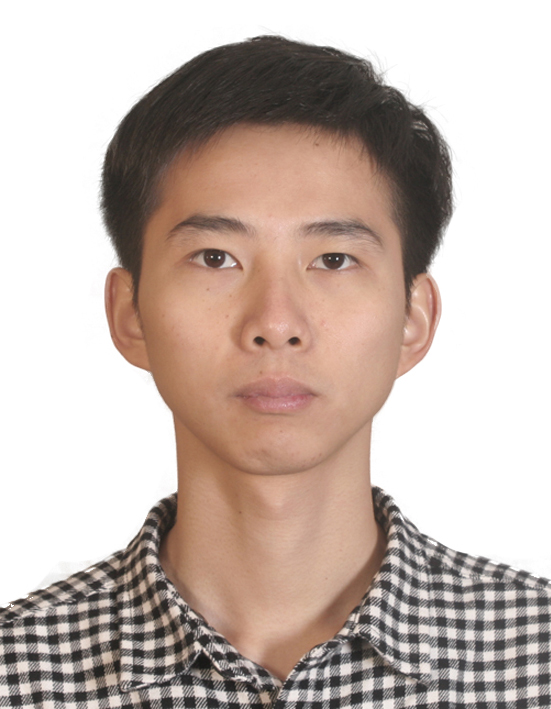
\includegraphics[width=1in,height=1.25in,clip,keepaspectratio]{J_Liu.jpg}}]%
{Jiaxiang Liu} received his B.S. degree from the School of Software,
Tsinghua University, China, in 2010. He is now a co-supervised
Ph.D. candidate between the Department of Computer Science and
Technology, Tsinghua University, China and LIX, \'Ecole Polytechnique,
France. His research interests include formal methods, rewrite systems
and embedded systems.
\end{IEEEbiography}

\begin{IEEEbiography}[{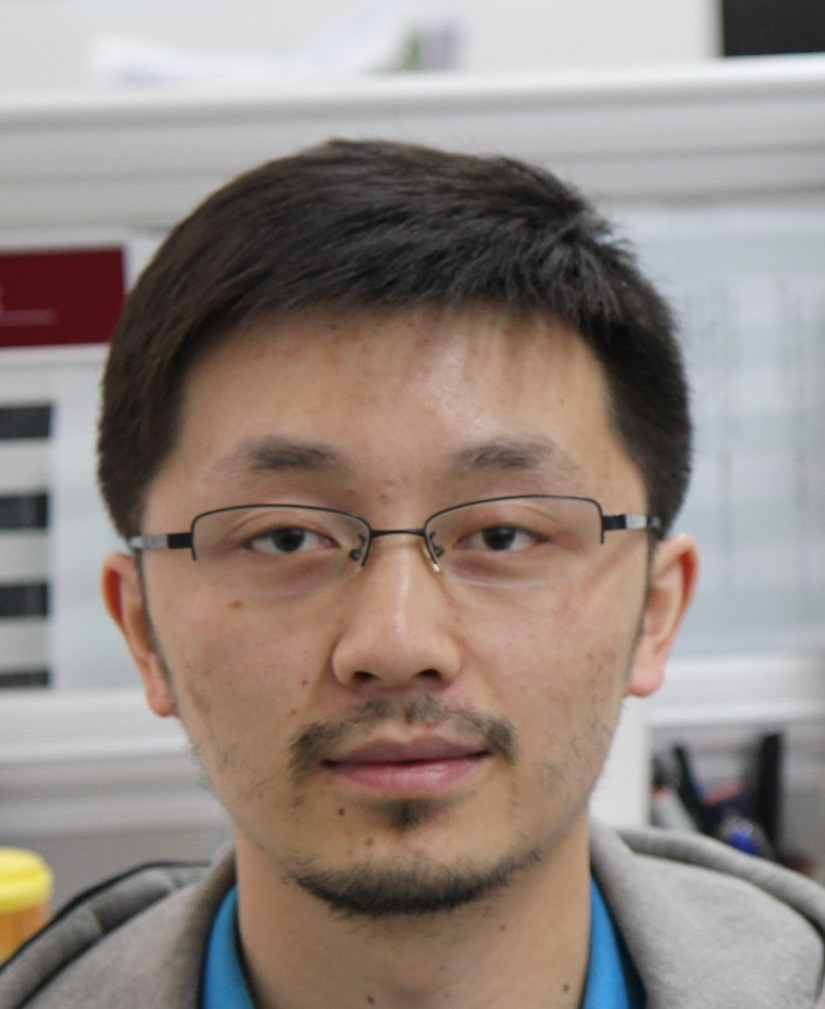
\includegraphics[width=1in,height=1.25in,clip,keepaspectratio]{M_Zhou.jpg}}]%
{Min Zhou} received his B.S. degree from the Department of
Mathematical Science and Ph.D. degree from the Department of Computer
Science and Technology, Tsinghua University, China, in 2007 and 2014,
respectively. He is now a lecturer at the School of Software, Tsinghua
University. His research interests include model checking, program
analysis and testing.
\end{IEEEbiography}

%% \vspace{-2cm}
\begin{IEEEbiography}[{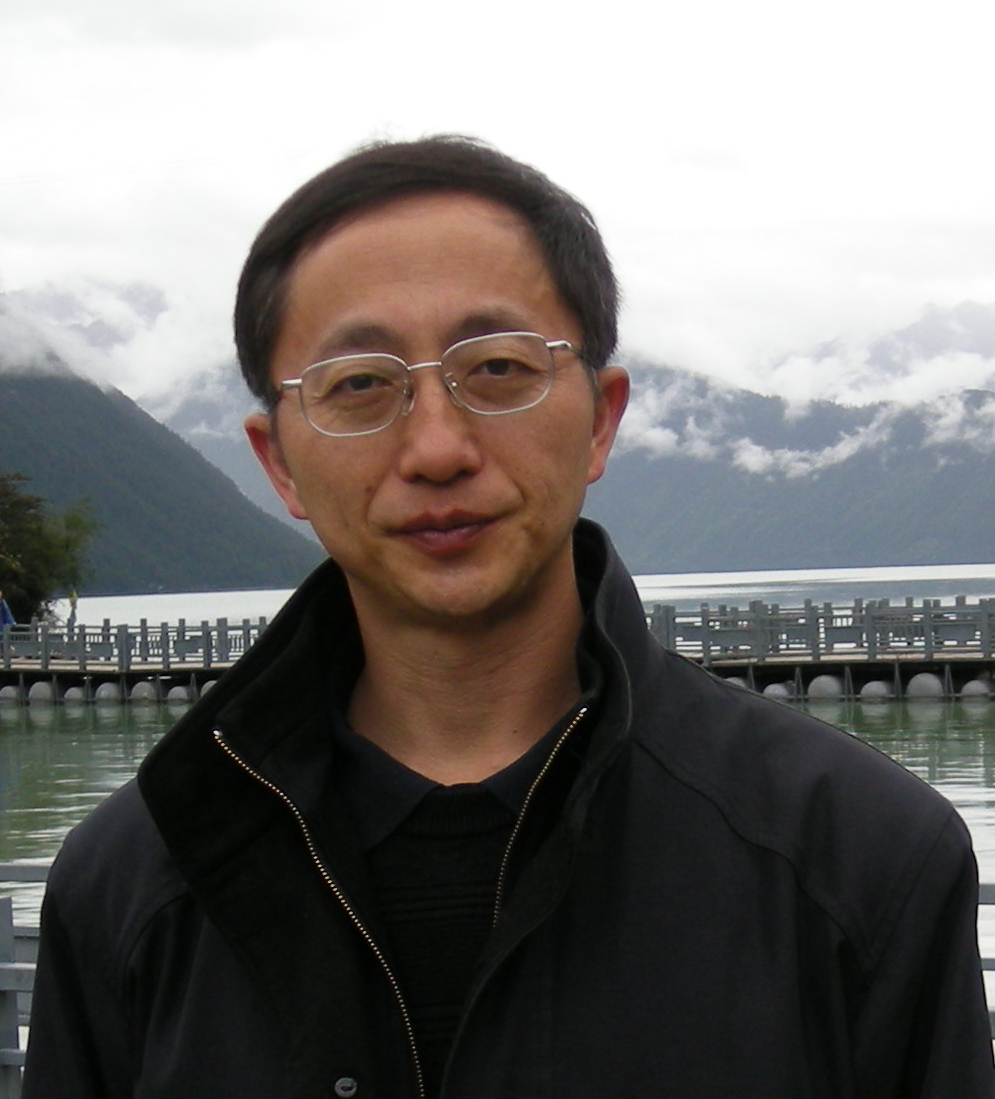
\includegraphics[width=1in,height=1.25in,clip,keepaspectratio]{X_Song.jpg}}]%
{Xiaoyu Song} () received the Ph.D. degree from the University of
Pisa, Italy, in 1991. From 1992 to 1998, he was on the faculty at the
University of Montreal, Canada. He joined the Department of Electrical
and Computer Engineering at Portland State University in 1998, where
he is now a professor. He was an editor of IEEE Transactions on VLSI
Systems and IEEE Transactions on Circuits and Systems. He was awarded
an Intel Faculty Fellowship from 2000 to 2005. His research interests
include formal methods, design automation, embedded systems and
emerging technologies.
\end{IEEEbiography}

\begin{IEEEbiography}[{
\includegraphics[width=1in,height=1.25in,clip,keepaspectratio]{M_Gu.jpg}}]%
{Ming Gu} is a professor at the School of Software, Tsinghua
University and vice-director of Ministry of Education Key Laboratory
of Information Security, China. Her research interests include
software formal methods, software trustworthiness and middleware
technology.
\end{IEEEbiography}

\begin{IEEEbiography}[{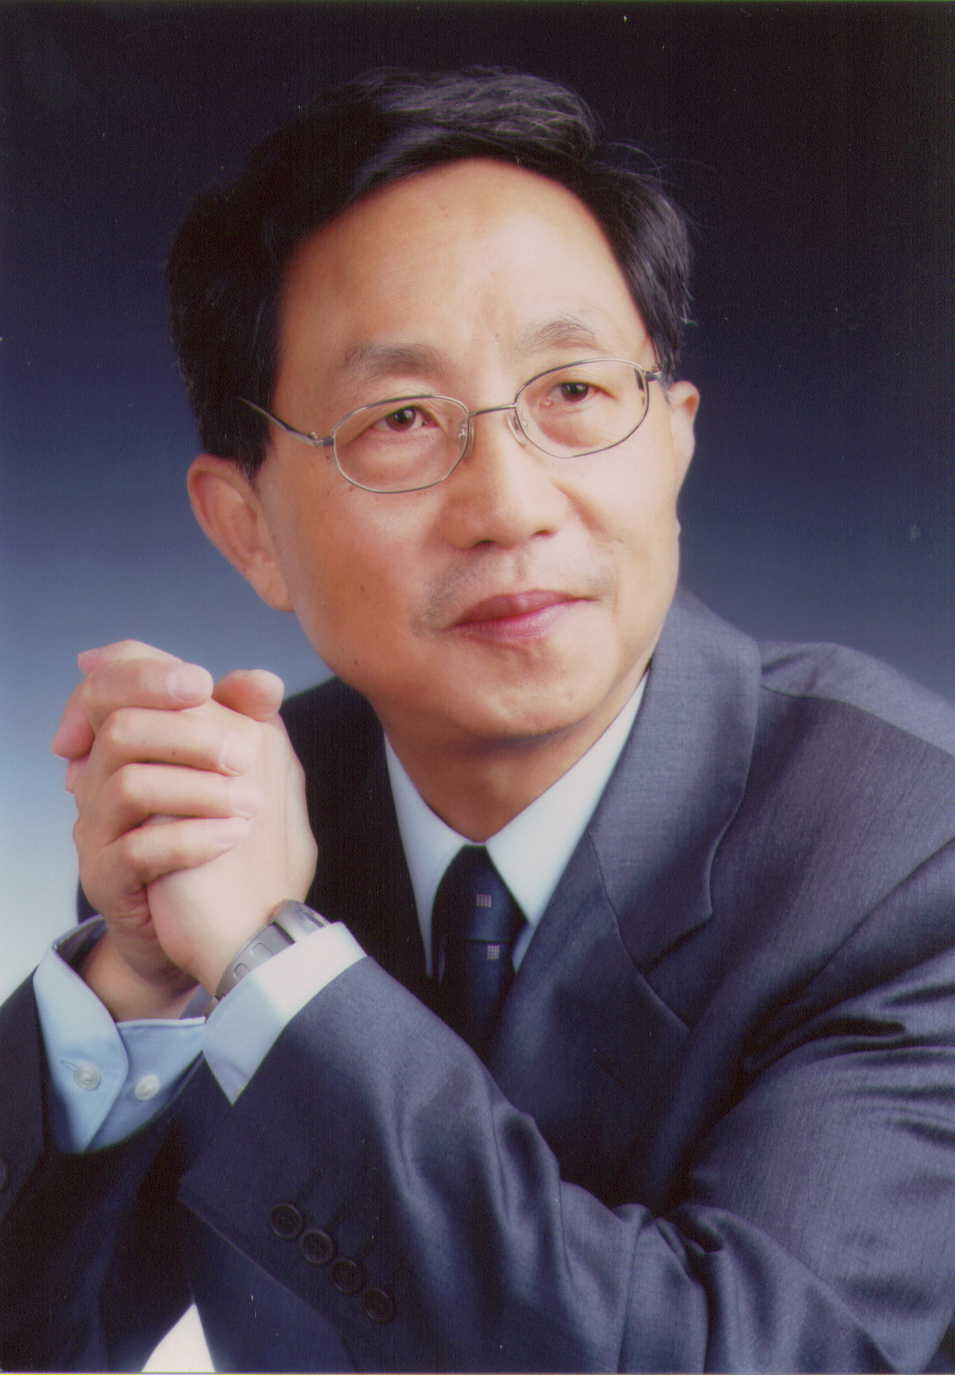
\includegraphics[width=1in,height=1.25in,clip,keepaspectratio]{J_Sun.jpg}}]%
{Jiaguang Sun} is a professor and dean of the School of Information
Science and Technology in Tsinghua University, China. He is also a
member of the Chinese Academy of Engineering, director of Ministry of
Education Key Laboratory of Information Security, and director of
Tsinghua National Laboratory for Information Science and Technology,
China. His research interests include computer graphics,
computer-aided design, formal verification of software, software
engineering, and system architecture.
\end{IEEEbiography}

\end{document}
